\documentclass[a4paper,11pt]{article}
\usepackage[T1]{fontenc}
\usepackage{lmodern}
\usepackage{babel}
\babelprovide[main,import]{spanish}
\usepackage[margin=2.5cm]{geometry}
\usepackage{microtype}
\usepackage{graphicx,xcolor,booktabs,array,tabularx,float,amsmath}
\usepackage[font=small,skip=6pt]{caption}
\usepackage{tikz}
\usetikzlibrary{arrows.meta,positioning,shapes.geometric}
\usepackage[hidelinks]{hyperref}

\hypersetup{
  pdftitle={SolarBell - Sistema de timbre automatizado con energía solar},
  pdfauthor={Andrés Felipe Ortiz Rodríguez, Néstor Junior Hernández López, José Enrique Otero Pineda, Julián Camilo Doria Guevara},
  pdfsubject={Informe final del Proyecto de Aula Semestral},
  bookmarksopen=true
}
\addto\captionsspanish{%
  \renewcommand{\contentsname}{Índice}%
  \renewcommand{\figurename}{Figura}%
  \renewcommand{\tablename}{Tabla}%
}
\setcounter{tocdepth}{2}
\setcounter{secnumdepth}{3}
\setlength{\parskip}{3.5pt plus 0.5pt}
\setlength{\parindent}{1.25em}
\setlength{\emergencystretch}{2em}
\renewcommand{\arraystretch}{1.09}
\raggedbottom
\urlstyle{same}
\definecolor{azulgris}{HTML}{536176}
\colorlet{linediag}{black!74}
\newcolumntype{Y}{>{\raggedright\arraybackslash}X}
\newcolumntype{P}[1]{>{\raggedright\arraybackslash}p{#1}}
\newcommand{\fuente}[1]{\par\smallskip{\centering\footnotesize #1\par}}
\newcommand{\seccionsinnumero}[1]{%
  \section*{#1}\phantomsection\addcontentsline{toc}{section}{#1}}
\newcommand{\senal}[1]{\texttt{#1}}
\newcommand{\bloquebiblio}[3]{\bibitem{#1} #2\par#3}
\newcommand{\enlaceanexo}[2]{\href{#1}{\textcolor{azulgris}{\underline{#2}}}}
\tikzset{
  cuadro/.style={draw=linediag,rounded corners=2pt,fill=black!3,
    align=center,minimum height=8mm,inner sep=4pt,font=\small},
  caso/.style={ellipse,draw=linediag,fill=black!3,align=center,
    text width=3.05cm,minimum height=10mm,inner sep=1pt,font=\small},
  flujo/.style={-{Stealth[length=2mm]},semithick,draw=linediag},
  linea/.style={semithick,draw=linediag},
  decision/.style={diamond,aspect=2.4,draw=linediag,fill=black!3,align=center,
    inner sep=1pt,font=\small},
  nota/.style={font=\footnotesize,fill=white,inner sep=2pt,align=center}
}

\begin{document}
\begin{titlepage}
\centering
\vspace*{1.12cm}
{\large\bfseries UNIVERSIDAD DE CÓRDOBA\par}
\vspace{0.27cm}
{\bfseries FACULTAD DE INGENIERÍA\par}
\vspace{0.25cm}
{\bfseries PROGRAMA DE INGENIERÍA DE SISTEMAS\par}
\vspace{0.25cm}
{\bfseries SEDE MONTERÍA\par}
\vfill
{\large\bfseries PROYECTO DE AULA SEMESTRAL --- INFORME FINAL\par}
\vspace{1.05cm}
{\LARGE\bfseries SolarBell\par}
\vspace{0.14cm}
{\LARGE\bfseries Sistema de timbre automatizado\par con energía solar\par}
\vspace{0.62cm}
{\color{azulgris}Control horario local, configuración desde Android\par
y activación manual por pulsador de pared\par}
\vfill
{\bfseries Presentado por\par}
\vspace{0.43cm}
Andrés Felipe Ortiz Rodríguez\par
Néstor Junior Hernández López\par
José Enrique Otero Pineda\par
Julián Camilo Doria Guevara\par
\vfill
{\bfseries Docentes\par}
\vspace{0.35cm}
Antonio Fernando Movilla Quintero\par
{\small Sistemas Operativos\par}
\vspace{0.21cm}
Milton Eduardo Hernández Zakzuk\par
{\small Arquitectura del Computador\par}
\vfill
{\bfseries Arquitectura del Computador y Sistemas Operativos\par}
\vspace{0.34cm}
Montería, noviembre de 2026\par
\vspace*{0.27cm}
\end{titlepage}

\pagenumbering{arabic}
\tableofcontents
\clearpage

% Introducción y resumen ejecutivo
\seccionsinnumero{Introducción}
El timbre escolar coordina la entrada a clase, los recesos y la finalización de la jornada. Cuando su manejo depende de una persona, cada aviso exige consultar la hora y accionar el pulsador en el momento previsto. A esto se añaden las jornadas con un horario distinto y los días en los que se suspenden los timbres ordinarios. La propuesta inicial del proyecto identificó estas dificultades y planteó automatizar los avisos con un ESP32, sincronización por Internet y seguimiento de la corriente de la carga \cite{propuesta}.

Durante el desarrollo cambió la forma de mantener la hora, configurar los repiques y alimentar la campana. La versión final, denominada SolarBell, utiliza un reloj DS3231SN y conserva el horario en el equipo. La aplicación Android pone en hora el reloj, se comunica con el ESP32 por Wi-Fi local y consulta el historial de los toques que el ESP32 anota en su memoria. La ruta automatizada obtiene energía del subsistema fotovoltaico con batería e inversor. En reposo, el pulsador conserva la ruta de activación mediante la red eléctrica escolar \cite{ficha,diagrama,evidencia}.

El prototipo se instaló en la Institución Educativa Cecilia de Lleras, en Montería. Las cuatro pruebas documentan el fallo inicial del LED que simulaba el timbre, el accionamiento del pulsador, la integración del módulo de relés y la verificación definitiva de un timbrado a la hora programada en la institución \cite{evidencia}.

Los cuatro objetivos específicos se alcanzaron. El ESP32, el reloj, la alimentación solar y los dos relés quedaron integrados en un solo equipo. El controlador ejecuta por sí solo el horario semanal y las fechas especiales. La aplicación Android pone en hora la campana, edita el calendario, ordena toques inmediatos y consulta el historial. Las cuatro pruebas quedaron documentadas en las evidencias fotográficas.

El informe presenta el problema, los objetivos y los antecedentes en tres contextos. La metodología expone la evolución del diseño. La arquitectura reúne los requisitos, los modelos de comportamiento y datos, y el desarrollo de hardware y software. Las pruebas se presentan con sus fotografías en el cuerpo del informe, seguidas de las conclusiones, las recomendaciones y los trabajos futuros. Al final, los anexos incluyen el manual del usuario, el manual del sistema, las evidencias fotográficas y el código fuente.

\seccionsinnumero{Resumen ejecutivo}
SolarBell es un prototipo académico de timbre automatizado para establecimientos educativos que utilizan avisos sonoros para coordinar su jornada. Su usuario directo es el personal encargado de ajustar horarios y realizar avisos extraordinarios. Los beneficiarios son docentes y estudiantes que reciben las señales de cambio de actividad.

Desde la aplicación Android se pueden definir horas de lunes a viernes, cantidad de toques, duración, pausas y fechas especiales. Cada fecha especial sustituye el horario semanal de ese día y puede dejarlo sin timbres. Al establecer la conexión, el teléfono actualiza la hora y la zona horaria. El equipo guarda el horario y lo ejecuta con su reloj local. También anota cada toque al terminar, y la aplicación permite consultar ese historial, buscarlo por nombre y filtrarlo por fecha. La aplicación se comunica con el ESP32 por HTTP, a través de la red SolarBell o de la red Wi-Fi del colegio, sin requerir Internet ni un servidor externo.

El ESP32 gobierna dos canales de relé. Uno energiza el inversor durante la secuencia y el otro acciona la campana toque por toque. Un panel de 30\,Wp, un controlador de carga y una batería de 12\,V y 7,5\,Ah forman el subsistema de alimentación solar. La ruta de pulsador físico sigue disponible en reposo cuando hay red eléctrica escolar \cite{ficha,diagrama}. La prueba definitiva en la Institución Educativa Cecilia de Lleras verificó la ejecución de un timbrado a la hora programada, según el reporte del equipo \cite{evidencia}.

El mercado son las instituciones educativas que hoy tocan el timbre a mano, en particular las que no cuentan con Internet estable o tienen cortes de energía, porque SolarBell no depende de Internet, de un servidor externo ni de la red eléctrica para los toques programados. Para instalarlo se requiere una campana de 110\,V con su pulsador de pared, un lugar soleado para el panel y un teléfono Android 7.0 o posterior. La red Wi-Fi de la institución es opcional y debe ser de 2,4\,GHz.

\clearpage
\section{Planteamiento del problema}
\subsection{Descripción del problema}
La jornada escolar se organiza mediante eventos que deben anunciarse en horas definidas. En una institución con timbre manual, la persona encargada del aviso debe conocer el horario vigente, estar disponible y accionar la campana en cada transición. El procedimiento es sencillo para un evento aislado, pero la repetición diaria aumenta la posibilidad de omisiones o atrasos. Si se programa una actividad especial, mantener el horario ordinario por error también puede interrumpir la jornada.

El control manual tiene un valor operativo propio. Ante una instrucción puntual, el personal puede pulsar el timbre de forma inmediata. Por ello, el proyecto contempla tanto la automatización habitual como el uso del pulsador de pared. En la propuesta inicial se planteó detectar si la campana consume corriente tras recibir una orden \cite{propuesta}. En la versión final, la aplicación muestra la conectividad, el reloj y la versión del programa, y consulta el historial de toques que el ESP32 guarda en su memoria. La comprobación eléctrica de la carga queda como una mejora posterior \cite{ficha,evidencia}.

\subsection{Justificación}
Guardar el horario en el dispositivo reduce la intervención necesaria para ejecutar los avisos recurrentes. El reloj dedicado permite conservar fecha y hora ante una interrupción de energía del control, y el manejo desde el teléfono facilita modificar el calendario desde el entorno del colegio. Las fechas especiales permiten ajustar un día concreto sin reescribir la programación semanal.

La alimentación fotovoltaica aporta una ruta automatizada con energía almacenada. La conmutación del inversor durante la secuencia evita mantenerlo activo permanentemente. Desde la perspectiva académica, el sistema integra comunicación por Wi-Fi y por bus I\textsuperscript{2}C, entradas y salidas digitales, almacenamiento de configuración y coordinación de eventos temporizados.

\section{Objetivos}
\subsection{General}
Desarrollar y documentar un prototipo de timbre escolar automatizado con ESP32, alimentación solar y reloj de tiempo real, configurable desde una aplicación Android en la red local y con una ruta de activación mediante pulsador de pared.

\subsection{Específicos}
\begin{enumerate}
  \item Integrar el ESP32, el reloj de tiempo real, la alimentación fotovoltaica y el módulo de dos relés en una arquitectura que controle el inversor y la campana.
  \item Organizar el control temporal para gestionar el horario semanal, las excepciones por fecha y la ejecución autónoma del patrón de repiques.
  \item Habilitar desde Android la puesta en hora, la gestión del calendario, el toque inmediato y la consulta del historial de toques que registra el ESP32.
  \item Documentar las cuatro pruebas, desde el fallo inicial del LED hasta el timbrado a la hora programada en la Institución Educativa Cecilia de Lleras.
\end{enumerate}

\clearpage
\section{Antecedentes}
\subsection{Contexto internacional}
Mahmood presenta un controlador de timbre escolar basado en ESP32 y un RTC DS3231. Su diseño emplea Wi-Fi para corregir la hora y Bluetooth para configurar el horario y otros parámetros. El antecedente ilustra la separación entre ajuste de calendario, conservación de la hora y accionamiento del timbre \cite{mahmood}.

En El Salvador, Flores Cortez y Cornejo instalaron entre 2014 y 2018 catorce timbres automatizados en escuelas públicas, sobre todo rurales. Cada equipo usa un Arduino UNO, un módulo Bluetooth HC-06, un relé de estado sólido y una aplicación hecha en App Inventor con la que el director modifica el horario. El trabajo muestra que un equipo de bajo costo, configurado desde el teléfono, resuelve el problema en escuelas con pocos recursos \cite{flores}.

SolarBell comparte la combinación de un microcontrolador y un reloj dedicado. En SolarBell, la puesta en hora procede del teléfono y la administración utiliza HTTP por Wi-Fi local. El proyecto incorpora además una ruta fotovoltaica para los repiques automatizados y un pulsador alimentado por la red escolar en reposo \cite{ficha,diagrama}.

\subsection{Contexto nacional}
En Boyacá, la Institución Educativa San Luis de Gaceno publicó un proyecto de timbre automatizado orientado a mejorar la puntualidad de los avisos y reducir las inconsistencias de la activación manual. Ese trabajo presenta un problema operativo comparable al de SolarBell: trasladar los avisos repetitivos de la jornada a un sistema programado \cite{gaceno}.

En la Universidad Popular del Cesar, seccional Aguachica, Badillo Rincón propuso una sirena escolar con Internet de las Cosas. Se configura desde un panel propio y desde una aplicación multiplataforma, permite tocar en tiempo real y lleva un registro de las jornadas para generar estadísticas \cite{badillo}.

Los antecedentes colombianos comparten el objetivo de ajustar los avisos a los tiempos de clase. En SolarBell, las fechas especiales permiten cambiar la programación de un solo día y el historial permite consultar desde la aplicación los toques que el equipo ejecutó \cite{ficha,repo}.

\subsection{Contexto regional}
En la Universidad de Córdoba, Yepes Mercado y Gómez Polo desarrollaron un timbre automatizado con luces LED para los estudiantes sordos de la Institución Educativa Santa Rosa de Lima, en Montería. El dispositivo señala los cambios de clase, los recesos y las emergencias de forma visual \cite{yepes}. Ese trabajo comparte con SolarBell la ciudad, el tipo de institución y la automatización de los avisos de la jornada. SolarBell se centra en el aviso sonoro, el calendario y la alimentación solar.

El caso regional propio de este informe corresponde a la Institución Educativa Cecilia de Lleras, en Montería, Córdoba. El equipo instaló allí SolarBell y realizó la prueba definitiva con un aviso a la hora programada. Durante la prueba en sitio se fotografió la aplicación en la vista del día, con la cuenta regresiva del próximo aviso \cite{evidencia}.

La instalación aplica el control horario a una carga puntual del establecimiento. El panel y la batería alimentan la ruta automatizada según el diseño, mientras el pulsador conserva el acceso a la campana desde la red de la institución. La prueba en sitio vincula la programación mostrada en Android con el uso del equipo en el colegio \cite{ficha,diagrama,evidencia}.

\begin{table}[H]
\centering\small
\caption{Relación de los antecedentes con SolarBell}
\begin{tabularx}{\linewidth}{@{}P{2.65cm}YY@{}}
\toprule
\textbf{Contexto} & \textbf{Aspecto relacionado} & \textbf{Aplicación en SolarBell} \\
\midrule
Internacional & Control de calendario con ESP32 y RTC. Timbres de bajo costo configurados desde el teléfono en escuelas rurales de El Salvador. & Reloj local con ajuste desde Android y equipo de bajo costo. \\
Nacional & Automatización de los avisos escolares en San Luis de Gaceno. Sirena con aplicación, toque en tiempo real y registro de jornadas en Aguachica. & Programación semanal, fechas especiales, toque inmediato e historial de toques. \\
Regional & Timbre con luces LED en la Institución Educativa Santa Rosa de Lima. Instalación propia en la Institución Educativa Cecilia de Lleras, Montería. & Automatización de los avisos en Montería y prueba de un timbrado a la hora programada en el sitio de estudio. \\
\bottomrule
\end{tabularx}
\end{table}

\clearpage
\section{Metodología}
\subsection{Tipo de trabajo}
El proyecto es de tipo tecnológico descriptivo. Su objeto es un prototipo que aplica hardware y software embebidos a una necesidad operativa escolar. La unidad de análisis es el prototipo junto con su aplicación Android y la ruta de pulsador físico. El sitio de estudio y de instalación fue la Institución Educativa Cecilia de Lleras, en Montería.

\subsection{Estrategias de recolección de la información}
La revisión documental se basó en la propuesta inicial, las fichas de hardware y software y el diagrama final. La propuesta identifica el punto de partida y las funciones previstas. La ficha describe las capacidades del equipo y el diagrama precisa las señales y los contactos de la ruta de potencia. Se utilizaron cuatro fotografías y las observaciones reportadas por el equipo, desde el fallo en el montaje inicial hasta la prueba en la institución. El código fuente del firmware y de la aplicación precisó el comportamiento de la versión final \cite{propuesta,ficha,diagrama,evidencia,repo}.

\begin{table}[H]
\centering\small
\caption{Fuentes empleadas en el análisis del prototipo}
\begin{tabularx}{\linewidth}{@{}P{3.3cm}YY@{}}
\toprule
\textbf{Fuente} & \textbf{Información extraída} & \textbf{Uso en el informe} \\
\midrule
Propuesta inicial & Problema, objetivos de arranque, NTP, panel web y diagnóstico por SCT-013. & Identificar el alcance previsto al inicio y las variaciones. \\
Ficha técnica final & Hardware, funciones móviles, calendario, puesta en hora y rutas de accionamiento. & Definir el alcance funcional de SolarBell. \\
Diagrama final & Contactos de los relés, señales GPIO, alimentación y protecciones dibujadas. & Interpretar el flujo eléctrico y explicar la conmutación. \\
Registro de pruebas & LED del ensayo inicial, pulsador, relés e instalación en Cecilia de Lleras. & Documentar la falla inicial y la validación en sitio. \\
Código fuente & Firmware 0.8.0 del ESP32 y aplicación Android de la rama \senal{main}, revisión \senal{0adeb14}. & Describir las rutas HTTP, las librerías, la persistencia y el historial. \\
\bottomrule
\end{tabularx}
\end{table}

\subsection{Proceso de la investigación}
\subsubsection{Fase I. Estudio, análisis e interpretación del sistema}
En esta fase se analizó la rutina que comienza con la definición de una hora y termina con el aviso audible. Se identificaron dos condiciones de uso: disparo recurrente según horario e intervención puntual mediante un mando. A partir de la propuesta se identificaron el ESP32, un elemento de potencia y una interfaz de administración como bloques funcionales del sistema.

El personal directivo, administrativo o de apoyo constituye la población usuaria porque administra el calendario o acciona el timbre. Los docentes y estudiantes reciben los avisos. Se distinguió al operador de la aplicación de quien usa el pulsador de pared, aunque ambos roles puedan recaer en la misma persona. Para el análisis se revisaron los documentos, se identificaron las funciones de cada componente y se consideró la prueba programada en la Institución Educativa Cecilia de Lleras. Las herramientas de esta fase fueron la revisión documental, la observación del montaje y de la institución, la fotografía de cada prueba y el monitor serie del entorno Arduino para leer los mensajes del ESP32. El código y los documentos se versionaron con Git en un repositorio de GitHub \cite{repo}.

\clearpage
\subsubsection{Fase II. Caracterización del sistema}
Se distinguieron tres orígenes para una activación: un evento programado, una orden inmediata enviada por Android y el pulsador de pared. Los dos primeros comparten la lógica de repiques y los relés del controlador. El tercero depende de la red escolar y actúa mediante la ruta de reposo del segundo canal. Esa diferencia permite entender qué funciones quedan disponibles cuando se desactiva la radio o se interrumpe la alimentación del ESP32 \cite{ficha,diagrama}.

El horario ordinario se define por días hábiles. Una fecha especial reemplaza la programación de esa fecha, incluso cuando su lista está vacía. La vista del día muestra la fecha local, los eventos aplicables y el próximo timbre. El reloj facilita al ESP32 decidir cuándo actuar. Al terminar cada toque, el controlador lo anota en su memoria con su origen y su resultado.

\subsubsection{Fase III. Diseño e implementación del sistema}
El diseño final distribuye el trabajo entre la aplicación Android, la lógica embebida, el RTC y la etapa de potencia. La aplicación consulta el estado, los horarios y el historial, y envía cambios u órdenes por HTTP local. El controlador almacena la programación y el historial, interpreta la hora y gobierna los GPIO de los dos canales \cite{ficha,diagrama,repo}.

El software se construyó con dos grupos de componentes. El firmware está escrito en C++ con el núcleo Arduino para ESP32 y usa las librerías de Wi-Fi, servidor web, mDNS, ArduinoJson, LittleFS, Preferences y RTClib (Tabla~\ref{tab:librerias}). La aplicación está escrita en TypeScript con React 19, Vite, React Router y Tailwind CSS, y Capacitor 8 la empaqueta como APK de Android. Ambos se comunican solo por la interfaz HTTP de la Tabla~\ref{tab:api}. La Tabla~\ref{tab:variaciones} resume cómo cambió el diseño frente a la propuesta.

\begin{table}[H]
\centering\small
\caption{Variaciones entre la propuesta y el sistema final}
\label{tab:variaciones}
\begin{tabularx}{\linewidth}{@{}P{2.35cm}YY@{}}
\toprule
\textbf{Aspecto} & \textbf{Propuesta inicial} & \textbf{Implementación documentada} \\
\midrule
Referencia horaria & Sincronización NTP por Wi-Fi. & RTC DS3231SN puesto en hora desde el teléfono. \\
Interfaz & Panel web, pantalla OLED y registro de incidencias. & Aplicación Android con agenda del día, estado e historial de timbrados realizados. \\
Patrones & Tres patrones predefinidos con duraciones fijas. & Cantidad, duración y pausa configurables por evento o toque inmediato. \\
Accionamiento manual & Pulsador como entrada del ESP32 con interrupción de hardware. & Pulsador de pared de 110\,V por la ruta de reposo. La app ofrece un mando inmediato independiente. \\
Potencia & Una etapa de relé para conmutar la campana. & Dos canales: uno para energizar el inversor y otro para accionar la campana. \\
Energía & Alimentación de la carga mediante conmutación de CA. & Panel, controlador PWM, batería e inversor para la operación automatizada. \\
Diagnóstico & Medición SCT-013 por ADC y alerta por ausencia de corriente. & Indicador visual en el circuito y lectura de estado desde la app. El monitoreo de corriente quedó fuera del alcance final. \\
\bottomrule
\end{tabularx}
\end{table}

\clearpage
\section{Diseño arquitectónico}
\subsection{Especificación y modelos}
La especificación parte de la ficha técnica, el flujo eléctrico del diagrama y el código del firmware y de la aplicación. Los modelos relacionan los actores, los datos y las salidas. Las denominaciones de clases y mensajes se usan como elementos del modelo.

\subsubsection{Requerimientos funcionales}
\begin{table}[H]
\centering\small
\caption{Requerimientos funcionales del sistema final}
\label{tab:rf}
\begin{tabularx}{\linewidth}{@{}P{1.33cm}P{3.02cm}Y@{}}
\toprule
\textbf{Código} & \textbf{Función} & \textbf{Comportamiento especificado} \\
\midrule
RF-01 & Establecer conexión & Comunicarse desde Android por HTTP mediante la red SolarBell o la red Wi-Fi del colegio. \\
RF-02 & Ajustar la hora & Aplicar la fecha, hora y zona del teléfono al establecer la conexión y conservar la referencia en el RTC. \\
RF-03 & Administrar el horario & Crear, modificar y eliminar eventos con nombre, hora, cantidad de repiques, duración y pausas, comunes o propias de cada toque. Mostrar los días activos del horario semanal, de lunes a viernes. Guardar la programación en el equipo. \\
RF-04 & Administrar fechas especiales & Crear, modificar y eliminar una fecha que sustituya el horario semanal por una programación propia o la deje sin timbrado. \\
RF-05 & Consultar día y estado & Mostrar la fecha, los timbres del día, el tiempo para el próximo aviso, las fechas especiales próximas, el alcance, el estado horario y la versión del programa. \\
RF-06 & Ejecutar eventos & Elegir la programación aplicable a la fecha y ejecutar el patrón cuando corresponda, incluso con la radio apagada. \\
RF-07 & Enviar y detener un toque & Iniciar un toque inmediato mediante Android con su patrón y solicitar la detención del toque en curso. \\
RF-08 & Activar por pulsador & Permitir el accionamiento de pared en reposo cuando hay red eléctrica escolar, con independencia del teléfono. \\
RF-09 & Controlar los dos canales & Alimentar el inversor durante la secuencia, conmutar la campana en cada toque y desconectar el inversor al terminar. \\
RF-10 & Ahorrar radio & Con el interruptor de Wi-Fi accionado, apagar la red propia SolarBell y conservar solo la unión a la red del colegio, o apagar el Wi-Fi si no hay red guardada. Conservar en ambos casos la ejecución del calendario almacenado. \\
RF-11 & Registrar timbrados & Anotar en el ESP32 cada toque al terminar, programado o inmediato, con su resultado: completo, detenido o reemplazado por otra orden. Consultar el historial desde la aplicación, buscarlo por nombre, filtrarlo por fecha y borrar registros. \\
\bottomrule
\end{tabularx}
\end{table}

La responsabilidad de crear un evento recae en la aplicación, mientras la ejecución del evento guardado recae en el controlador. Si el teléfono está fuera de alcance, el cambio de horario no se guarda en la campana \cite{ficha}. Esta condición determina el comportamiento de la consulta remota y la continuidad del calendario local.

\clearpage
\subsubsection{Requerimientos no funcionales}
\begin{table}[H]
\centering\small
\caption{Condiciones de operación y atributos de calidad}
\label{tab:rnf}
\begin{tabularx}{\linewidth}{@{}P{1.44cm}P{2.8cm}Y@{}}
\toprule
\textbf{Código} & \textbf{Atributo} & \textbf{Condición del diseño} \\
\midrule
RNF-01 & Autonomía operativa & La ejecución de la programación guardada depende del reloj local y de la alimentación del equipo. \\
RNF-02 & Operación local & La administración funciona mediante la conexión Wi-Fi local. La plataforma de la aplicación es Android. \\
RNF-03 & Conservación de datos & El dispositivo conserva el horario y el historial en su memoria flash, y el RTC conserva fecha y hora ante la pérdida de alimentación principal. El historial guarda hasta 1.000 toques y descarta los más antiguos. \\
RNF-04 & Uso de energía & El inversor permanece apagado en reposo. El interruptor de Wi-Fi suprime la red propia, que es lo que más consume, y deja la radio en reposo entre balizas del router. \\
RNF-05 & Operación manual & La ruta de pared está prevista para funcionar con el controlador apagado si se dispone de red escolar. \\
RNF-06 & Observabilidad & El operador puede consultar alcance, condición de hora, versión e historial de los timbrados realizados en el ESP32. \\
\bottomrule
\end{tabularx}
\end{table}

\subsubsection{Diagramas de caso de uso}
El operador de Android administra el calendario, consulta el día y el historial y solicita toques. El usuario del pulsador interactúa con el circuito de pared. El RTC aporta la referencia temporal para la ejecución autónoma, representada en los diagramas de secuencia y actividades.

\begin{figure}[H]
\centering
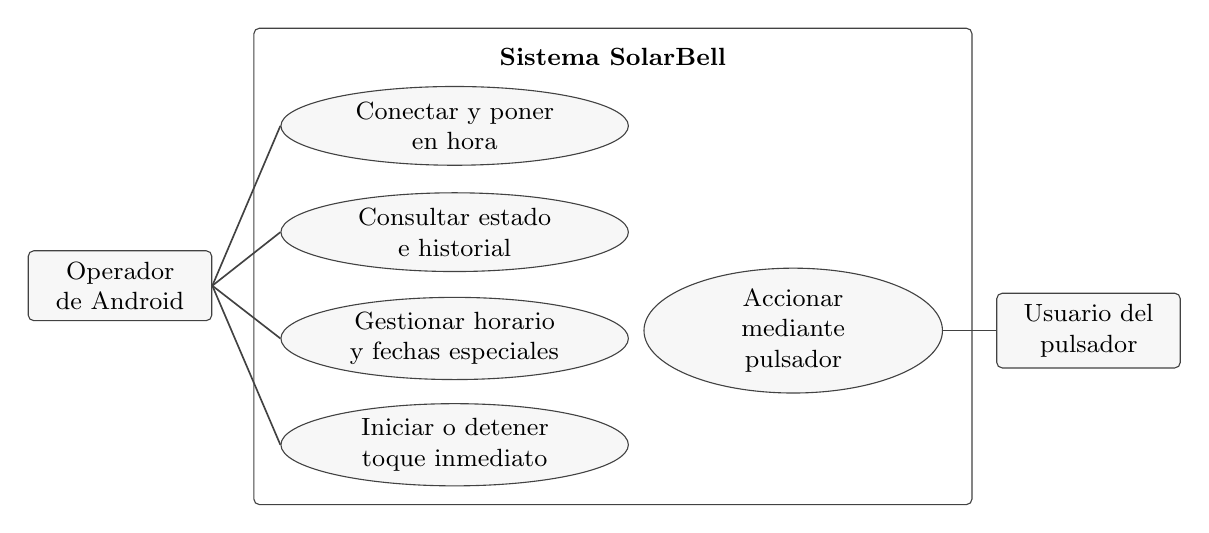
\begin{tikzpicture}
  \draw[linediag,rounded corners=2pt] (-4.45,-3.11) rectangle (4.67,2.94);
  \node[font=\small\bfseries] at (0.11,2.58) {Sistema SolarBell};
  \node[cuadro,text width=2.05cm] (app) at (-6.15,-0.33) {Operador de Android};
  \node[cuadro,text width=2.05cm] (pared) at (6.15,-0.90) {Usuario del pulsador};
  \node[caso] (hora) at (-1.90,1.70) {Conectar y poner\par en hora};
  \node[caso] (estado) at (-1.90,0.35) {Consultar estado\par e historial};
  \node[caso] (agenda) at (-1.90,-1.00) {Gestionar horario\par y fechas especiales};
  \node[caso] (toque) at (-1.90,-2.35) {Iniciar o detener\par toque inmediato};
  \node[caso,text width=2.61cm] (fisico) at (2.40,-0.90) {Accionar mediante\par pulsador};
  \draw[linea] (app.east) -- (hora.west);
  \draw[linea] (app.east) -- (estado.west);
  \draw[linea] (app.east) -- (agenda.west);
  \draw[linea] (app.east) -- (toque.west);
  \draw[linea] (pared.west) -- (fisico.east);
\end{tikzpicture}
\caption{Casos de uso según el medio de interacción}
\label{fig:casos}
\fuente{Elaboración propia a partir de la ficha técnica y del diagrama final.}
\end{figure}

\clearpage
\subsubsection{Diagramas de clase}
El modelo de clases describe la configuración y su relación con el control. \textit{Evento de timbre} agrupa una hora, un nombre y un patrón. El horario semanal indica los días activos, comunes a todos sus eventos. Una fecha especial tiene una fecha, un nombre, un modo y una lista propia. Cada atributo muestra el tipo y el rango que acepta el firmware. En la ejecución, el controlador consulta el calendario y el reloj y utiliza los canales de potencia. Los nombres y cardinalidades representan el dominio funcional.

\begin{figure}[H]
\centering
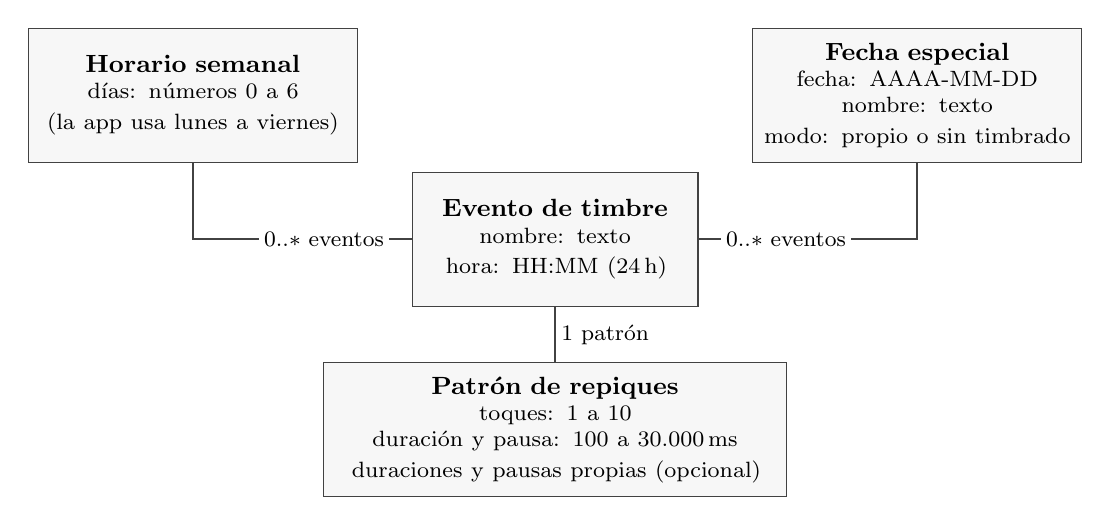
\begin{tikzpicture}[
  clase/.style={draw=linediag,align=center,inner sep=4pt,minimum height=17mm,
    text width=3.35cm,font=\small,fill=black!3},
  control/.style={clase,minimum height=14mm}
]
  \node[clase,text width=3.9cm] (semana) at (-4.6,0) {\textbf{Horario semanal}\par\footnotesize días: números 0 a 6\par (la app usa lunes a viernes)};
  \node[clase,text width=3.9cm] (fecha) at (4.6,0) {\textbf{Fecha especial}\par\footnotesize fecha: AAAA-MM-DD\par nombre: texto\par modo: propio o sin timbrado};
  \node[clase] (evento) at (0,-1.83) {\textbf{Evento de timbre}\par\footnotesize nombre: texto\par hora: HH:MM (24\,h)};
  \node[clase,text width=5.6cm] (patron) at (0,-4.25) {\textbf{Patrón de repiques}\par\footnotesize toques: 1 a 10\par duración y pausa: 100 a 30.000\,ms\par duraciones y pausas propias (opcional)};
  \draw[linea] (semana.south) |- node[pos=.80,nota] {$0..*$ eventos} (evento.west);
  \draw[linea] (fecha.south) |- node[pos=.80,nota] {$0..*$ eventos} (evento.east);
  \draw[linea] (evento.south) -- node[right,nota] {1 patrón} (patron.north);
\end{tikzpicture}
\caption{Modelo de clases del calendario y del patrón de repiques}
\label{fig:clasesagenda}
\end{figure}

\begin{figure}[H]
\centering
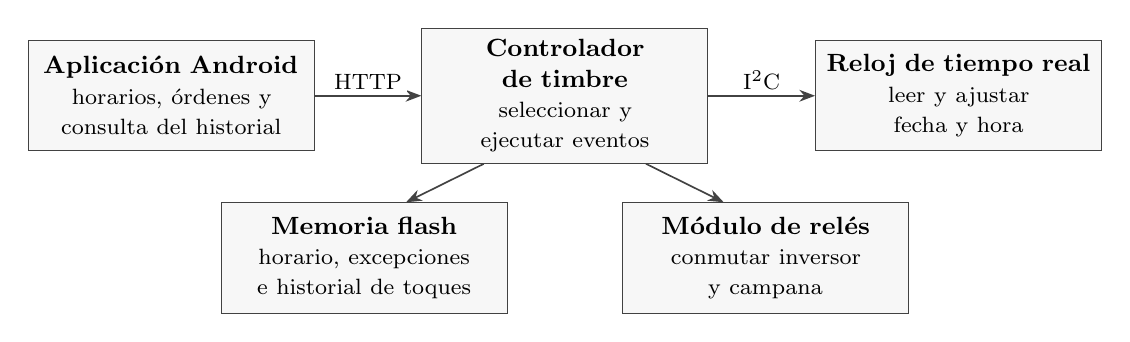
\begin{tikzpicture}[
  clase/.style={draw=linediag,align=center,inner sep=4pt,minimum height=14mm,
    text width=3.35cm,font=\small,fill=black!3}
]
  \node[clase] (app) at (-5.0,0) {\textbf{Aplicación Android}\par\footnotesize horarios, órdenes y consulta del historial};
  \node[clase] (esp) at (0,0) {\textbf{Controlador de timbre}\par\footnotesize seleccionar y ejecutar eventos};
  \node[clase] (rtc) at (5.0,0) {\textbf{Reloj de tiempo real}\par\footnotesize leer y ajustar fecha y hora};
  \node[clase] (cal) at (-2.55,-2.06) {\textbf{Memoria flash}\par\footnotesize horario, excepciones e historial de toques};
  \node[clase] (reles) at (2.55,-2.06) {\textbf{Módulo de relés}\par\footnotesize conmutar inversor y campana};
  \draw[flujo] (app.east) -- node[above,nota] {HTTP} (esp.west);
  \draw[flujo] (esp.east) -- node[above,nota] {I\textsuperscript{2}C} (rtc.west);
  \draw[flujo] (esp.220) -- (cal.53);
  \draw[flujo] (esp.320) -- (reles.127);
\end{tikzpicture}
\caption{Clases de control e interfaces principales}
\label{fig:clasescontrol}
\fuente{Modelos elaborados a partir de la ficha de software y el diagrama del circuito.}
\end{figure}

El patrón es un dato común a la programación y al toque inmediato. El evento programado añade la hora que lo vincula al calendario. El controlador cuenta los repiques y respeta sus pausas. El RTC suministra fecha y hora, el módulo de relés ejecuta las órdenes eléctricas y la memoria flash conserva el calendario y el historial que la aplicación consulta.

\clearpage
\subsubsection{Diagramas de secuencia}
En la configuración desde el teléfono, la escritura del horario es una operación sobre el ESP32. La interfaz móvil transmite el cambio y el reloj mantiene la referencia temporal. En el esquema, la respuesta resume el intercambio HTTP entre la aplicación y el equipo \cite{ficha}.

\begin{figure}[H]
\centering
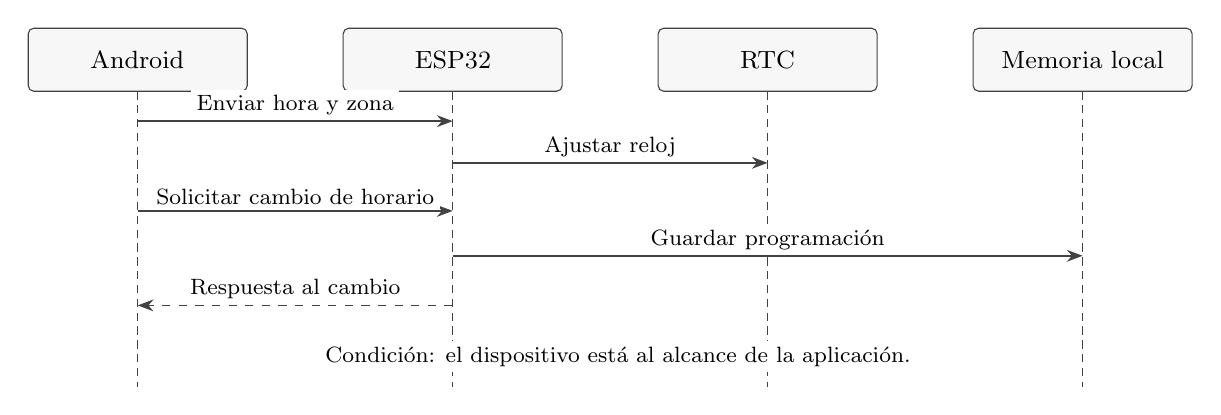
\begin{tikzpicture}[instancia/.style={cuadro,text width=2.5cm}]
  \node[instancia] at (0,0) {Android};
  \node[instancia] at (4,0) {ESP32};
  \node[instancia] at (8,0) {RTC};
  \node[instancia] at (12,0) {Memoria local};
  \foreach \x in {0,4,8,12} \draw[linediag,densely dashed] (\x,-.4) -- (\x,-4.15);
  \draw[flujo] (0,-.78) -- node[above,nota] {Enviar hora y zona} (4,-.78);
  \draw[flujo] (4,-1.31) -- node[above,nota] {Ajustar reloj} (8,-1.31);
  \draw[flujo] (0,-1.92) -- node[above,nota] {Solicitar cambio de horario} (4,-1.92);
  \draw[flujo] (4,-2.49) -- node[above,nota] {Guardar programación} (12,-2.49);
  \draw[flujo,dashed] (4,-3.12) -- node[above,nota] {Respuesta al cambio} (0,-3.12);
  \node[nota] at (6.1,-3.77) {Condición: el dispositivo está al alcance de la aplicación.};
\end{tikzpicture}
\caption{Puesta en hora y actualización del horario desde Android}
\label{fig:seqconfig}
\end{figure}

En un toque programado, la acción empieza cuando la hora coincide con un evento aplicable. El canal 1 alimenta el inversor durante la secuencia completa. El canal 2 alterna entre repique y pausa según el patrón. Al concluir, la salida de control del inversor vuelve a reposo \cite{diagrama}.

\begin{figure}[H]
\centering
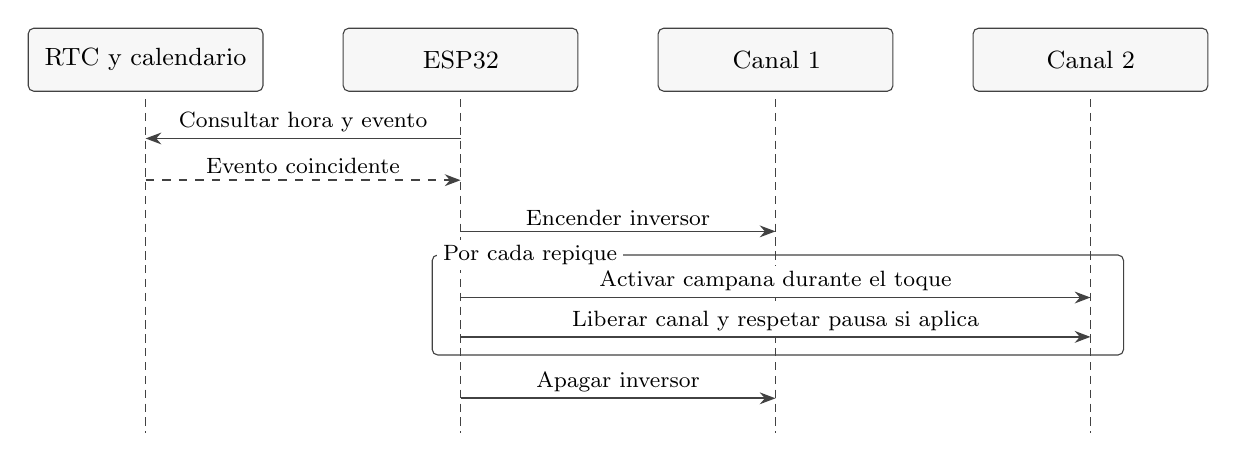
\begin{tikzpicture}[instancia/.style={cuadro,text width=2.70cm}]
  \node[instancia] at (0,0) {RTC y calendario};
  \node[instancia] at (4,0) {ESP32};
  \node[instancia] at (8,0) {Canal 1};
  \node[instancia] at (12,0) {Canal 2};
  \foreach \x in {0,4,8,12} \draw[linediag,densely dashed] (\x,-.5) -- (\x,-4.74);
  \draw[flujo] (4,-1.00) -- node[above,nota] {Consultar hora y evento} (0,-1.00);
  \draw[flujo,dashed] (0,-1.53) -- node[above,nota] {Evento coincidente} (4,-1.53);
  \draw[flujo] (4,-2.18) -- node[above,nota] {Encender inversor} (8,-2.18);
  \draw[rounded corners=2pt,linediag] (3.64,-2.48) rectangle (12.42,-3.75);
  \node[nota,anchor=west] at (3.70,-2.48) {Por cada repique};
  \draw[flujo] (4,-3.02) -- node[above,nota] {Activar campana durante el toque} (12,-3.02);
  \draw[flujo] (4,-3.52) -- node[above,nota] {Liberar canal y respetar pausa si aplica} (12,-3.52);
  \draw[flujo] (4,-4.30) -- node[above,nota] {Apagar inversor} (8,-4.30);
\end{tikzpicture}
\caption{Ejecución de un toque programado}
\label{fig:seqejec}
\end{figure}

El toque inmediato de Android aporta el patrón directamente al controlador. La orden de detención corta el toque en curso y una orden nueva lo reemplaza. En los tres desenlaces, el ESP32 anota el toque en el historial al terminar, con el tiempo que sonó de verdad. Un corte de energía a mitad del toque no deja registro. La aplicación lee el historial bajo demanda y lo vuelve a pedir cuando el estado informa un registro nuevo. El pulsador de pared sigue una trayectoria eléctrica independiente de esta secuencia y no queda en el historial \cite{repo}.

\begin{figure}[H]
\centering
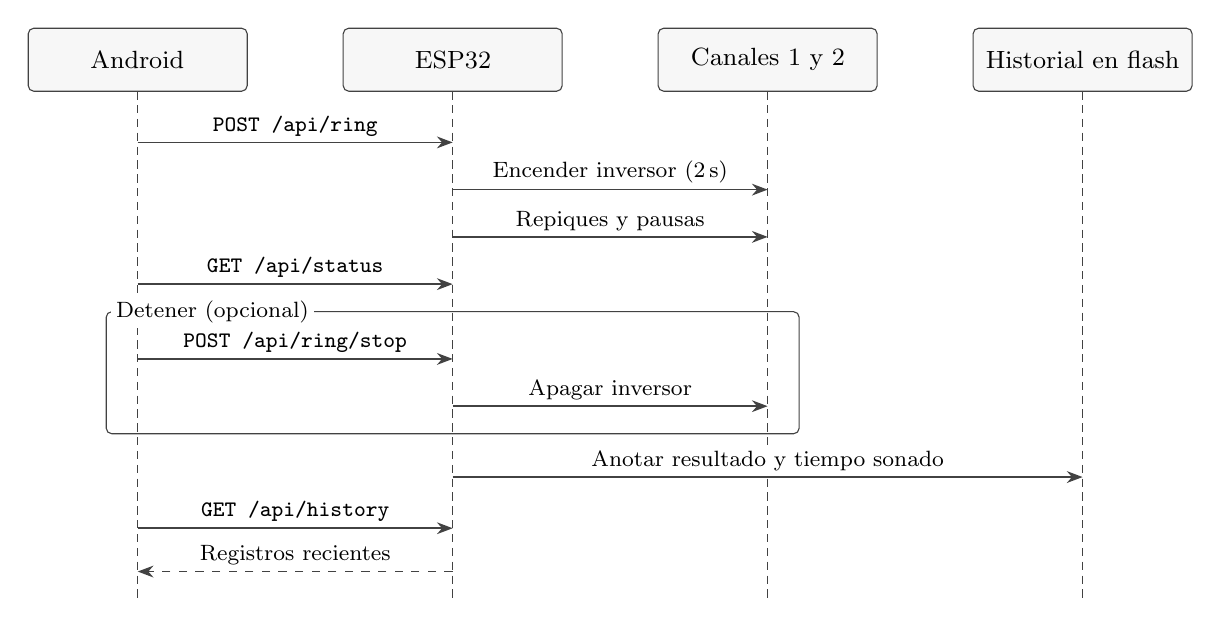
\begin{tikzpicture}[instancia/.style={cuadro,text width=2.5cm}]
  \node[instancia] at (0,0) {Android};
  \node[instancia] at (4,0) {ESP32};
  \node[instancia] at (8,0) {Canales 1 y 2};
  \node[instancia] at (12,0) {Historial en flash};
  \foreach \x in {0,4,8,12} \draw[linediag,densely dashed] (\x,-.4) -- (\x,-6.85);
  \draw[flujo] (0,-1.05) -- node[above,nota] {\senal{POST /api/ring}} (4,-1.05);
  \draw[flujo] (4,-1.65) -- node[above,nota] {Encender inversor (2\,s)} (8,-1.65);
  \draw[flujo] (4,-2.25) -- node[above,nota] {Repiques y pausas} (8,-2.25);
  \draw[flujo] (0,-2.85) -- node[above,nota] {\senal{GET /api/status}} (4,-2.85);
  \draw[rounded corners=2pt,linediag] (-0.40,-3.20) rectangle (8.40,-4.75);
  \node[nota,anchor=west] at (-0.35,-3.20) {Detener (opcional)};
  \draw[flujo] (0,-3.80) -- node[above,nota] {\senal{POST /api/ring/stop}} (4,-3.80);
  \draw[flujo] (4,-4.40) -- node[above,nota] {Apagar inversor} (8,-4.40);
  \draw[flujo] (4,-5.30) -- node[above,nota] {Anotar resultado y tiempo sonado} (12,-5.30);
  \draw[flujo] (0,-5.95) -- node[above,nota] {\senal{GET /api/history}} (4,-5.95);
  \draw[flujo,dashed] (4,-6.50) -- node[above,nota] {Registros recientes} (0,-6.50);
\end{tikzpicture}
\caption{Toque inmediato, detención y registro en el historial}
\label{fig:seqtoque}
\end{figure}

\clearpage
\subsubsection{Diagramas de actividades}
El flujo automático parte del día y la hora del RTC. Una excepción por fecha se evalúa antes de consultar el horario semanal. Si la excepción está vacía, se mantiene el día sin avisos automáticos. La salida programada se produce cuando el evento de la lista aplicable coincide con la hora de ejecución.

\begin{figure}[H]
\centering
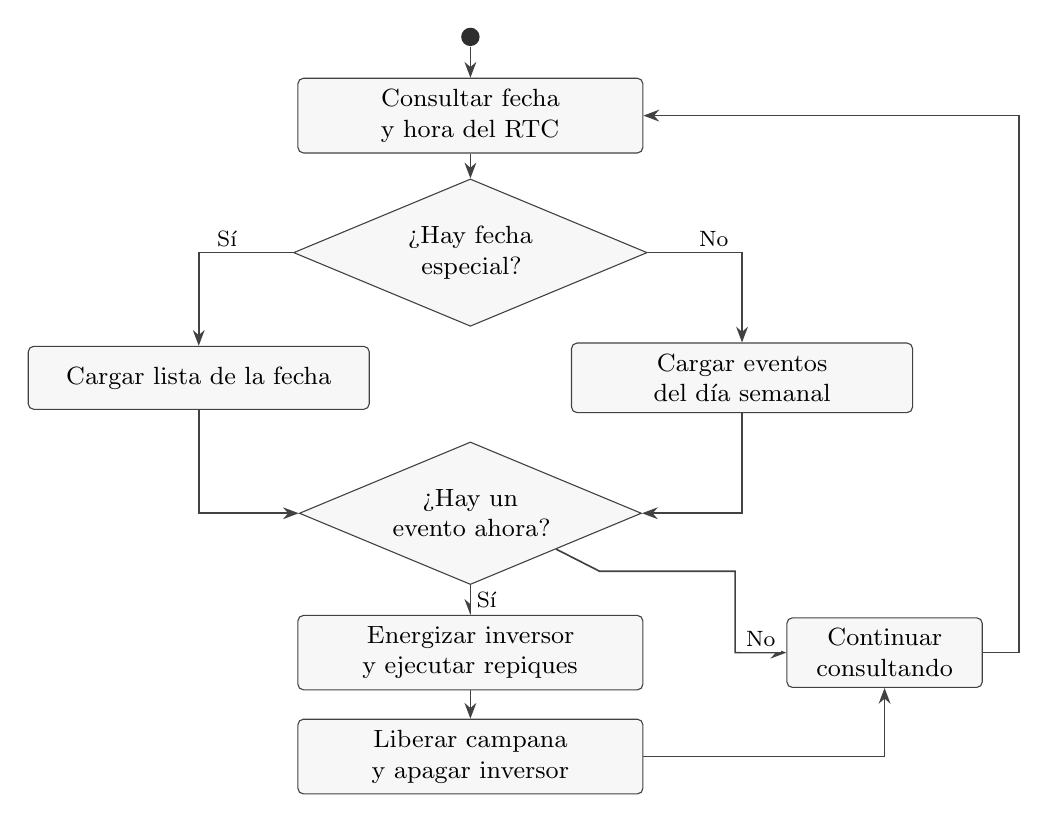
\begin{tikzpicture}
  \node[circle,fill=black!82,inner sep=2.35pt] (inicio) at (0,0) {};
  \node[cuadro,text width=4.1cm] (leer) at (0,-1.00) {Consultar fecha y hora del RTC};
  \node[decision,text width=2.65cm] (ex) at (0,-2.74) {¿Hay fecha especial?};
  \node[cuadro,text width=4.05cm] (listar) at (-3.45,-4.33) {Cargar lista de la fecha};
  \node[cuadro,text width=4.05cm] (sem) at (3.45,-4.33) {Cargar eventos del día semanal};
  \node[decision,text width=2.66cm] (coinc) at (0,-6.05) {¿Hay un evento ahora?};
  \node[cuadro,text width=4.1cm] (on) at (0,-7.82) {Energizar inversor y ejecutar repiques};
  \node[cuadro,text width=4.1cm] (off) at (0,-9.14) {Liberar campana y apagar inversor};
  \node[cuadro,text width=2.2cm] (esperar) at (5.26,-7.82) {Continuar consultando};
  \draw[flujo] (inicio) -- (leer);
  \draw[flujo] (leer) -- (ex);
  \draw[flujo] (ex.west) -| node[pos=.35,above,nota] {Sí} (listar.north);
  \draw[flujo] (ex.east) -| node[pos=.35,above,nota] {No} (sem.north);
  \draw[flujo] (listar.south) |- (coinc.west);
  \draw[flujo] (sem.south) |- (coinc.east);
  \draw[flujo] (coinc.south) -- node[right,nota] {Sí} (on.north);
  \draw[flujo] (coinc.south east) -- ++(.55,-.28) -| ([xshift=-.65cm]esperar.west)
    -- node[above,nota] {No} (esperar.west);
  \draw[flujo] (on) -- (off);
  \draw[flujo] (off.east) -| (esperar.south);
  \draw[flujo] (esperar.east) -- ++(.46,0) |- (leer.east);
\end{tikzpicture}
\caption{Flujo de decisión del timbrado automático}
\label{fig:actividad}
\end{figure}

\begin{table}[H]
\centering\small
\caption{Precedencia para la selección de avisos automáticos}
\begin{tabularx}{\linewidth}{@{}P{5.4cm}Y@{}}
\toprule
\textbf{Condición de la fecha consultada} & \textbf{Programación aplicable} \\
\midrule
Existe fecha especial con horario propio y repiques. & Se consideran los eventos de esa fecha. \\
Existe fecha especial sin timbrado o con lista vacía. & El día queda sin timbres automáticos. Los eventos guardados en una fecha sin timbrado se conservan por si vuelve a horario propio. \\
La fecha no es especial y el día tiene eventos semanales. & Se consideran los eventos habilitados para ese día. \\
El día está fuera del horario semanal y no tiene excepción. & No hay eventos automáticos para la fecha. \\
\bottomrule
\end{tabularx}
\end{table}

Al editar el horario, la aplicación muestra el cambio de inmediato y envía el horario completo a la campana. Si hay varios cambios seguidos, los envía en orden para que la campana guarde el último. Si la campana no confirma, la aplicación avisa del error y vuelve a la última versión que la campana sí guardó, de modo que la pantalla nunca muestra un horario que el equipo no tiene \cite{repo}.

\begin{figure}[H]
\centering
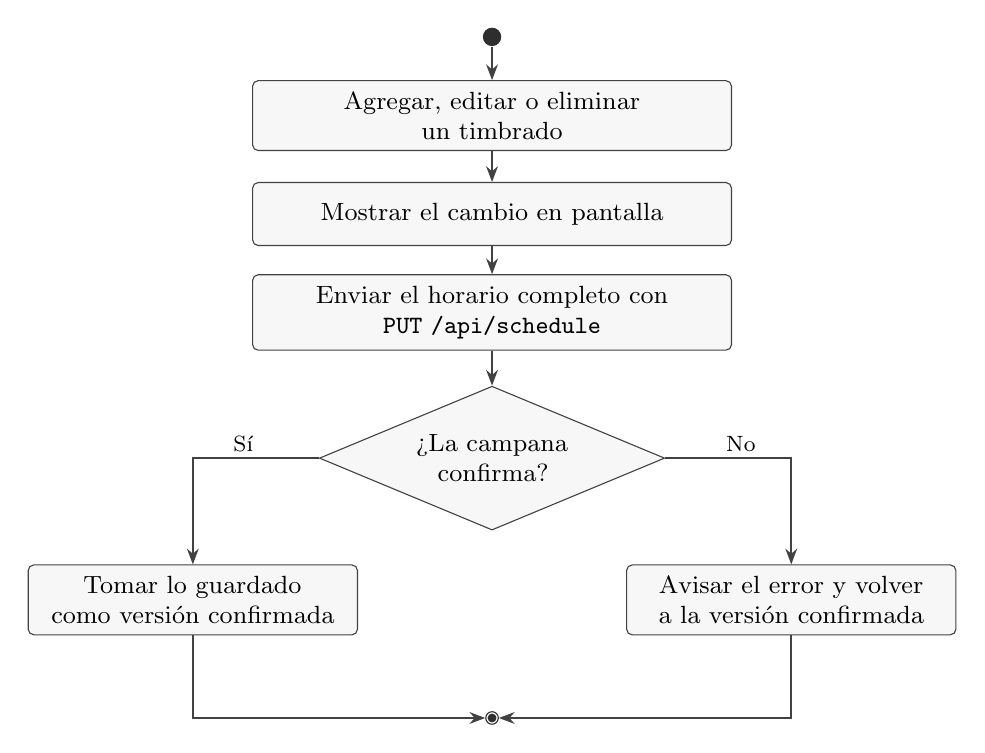
\begin{tikzpicture}
  \node[circle,fill=black!82,inner sep=2.35pt] (inicio) at (0,0) {};
  \node[cuadro,text width=5.8cm] (editar) at (0,-1.00) {Agregar, editar o eliminar\\un timbrado};
  \node[cuadro,text width=5.8cm] (mostrar) at (0,-2.25) {Mostrar el cambio en pantalla};
  \node[cuadro,text width=5.8cm] (enviar) at (0,-3.50) {Enviar el horario completo con\\\senal{PUT /api/schedule}};
  \node[decision,text width=2.7cm] (ok) at (0,-5.35) {¿La campana confirma?};
  \node[cuadro,text width=3.9cm] (guardar) at (-3.8,-7.15) {Tomar lo guardado como versión confirmada};
  \node[cuadro,text width=3.9cm] (volver) at (3.8,-7.15) {Avisar el error y volver a la versión confirmada};
  \node[circle,draw=black!82,inner sep=1.6pt,fill=white] (fin) at (0,-8.65) {};
  \fill[black!82] (fin) circle (1.6pt);
  \draw[flujo] (inicio) -- (editar);
  \draw[flujo] (editar) -- (mostrar);
  \draw[flujo] (mostrar) -- (enviar);
  \draw[flujo] (enviar) -- (ok);
  \draw[flujo] (ok.west) -| node[pos=.3,above,nota] {Sí} (guardar.north);
  \draw[flujo] (ok.east) -| node[pos=.3,above,nota] {No} (volver.north);
  \draw[flujo] (guardar.south) |- (fin.west);
  \draw[flujo] (volver.south) |- (fin.east);
\end{tikzpicture}
\caption{Edición del horario desde Android}
\label{fig:actividadedicion}
\fuente{Elaboración propia a partir del código de la aplicación \cite{repo}.}
\end{figure}

\clearpage
\subsubsection{Diseño de la base de datos}
La programación completa se guarda en la memoria de la campana y la aplicación se comunica directamente con el equipo \cite{ficha}. No hay un motor de base de datos. El ESP32 usa el sistema de archivos LittleFS sobre la partición de datos de su flash, de 1.408\,KB, y la biblioteca \textit{Preferences} para pares clave--valor. El teléfono solo guarda copias de consulta y preferencias de la interfaz \cite{repo}.

\begin{table}[H]
\centering\small
\caption{Dónde y con qué formato se guarda cada dato}
\label{tab:persistencia}
\begin{tabularx}{\linewidth}{@{}P{2.9cm}P{3.6cm}Y@{}}
\toprule
\textbf{Dato} & \textbf{Lugar y formato} & \textbf{Detalle} \\
\midrule
Horario y fechas especiales & ESP32, archivo \senal{/horario.json} en LittleFS. & Documento JSON con \senal{weekly} (días y eventos) y \senal{specials}. Cada escritura completa sube \senal{scheduleRevision}. Tamaño máximo de 24\,KB. \\
Historial de toques & ESP32, archivos binarios de 40 registros en LittleFS. & Registro fijo de 96\,B: hora de la orden, ms sonados, origen, resultado, hasta 10 duraciones, 9 pausas y el nombre. Hasta 25 archivos, unos 1.000 registros y el 7\,\% de la partición. Al abrir el archivo 26 se borra el más antiguo. \\
Red del colegio, zona horaria y último minuto tocado & ESP32, \textit{Preferences} en la flash. & Nombre y clave de la red elegida desde la app, desfase en minutos y el minuto del último timbrado, para no repetirlo tras un reinicio. \\
Fecha y hora & RTC DS3231SN con su batería de respaldo. & El ESP32 la lee por I\textsuperscript{2}C al arrancar. La app la corrige si difiere en más de 5\,s. \\
Copia del horario, último patrón manual, dirección de la campana y tema & Teléfono, \senal{localStorage} de la aplicación. & Solo sirven para mostrar datos mientras llega la respuesta y para encontrar la campana. La referencia es siempre la campana. \\
\bottomrule
\end{tabularx}
\end{table}

El historial solo agrega registros, para no desgastar la flash reescribiendo un mismo archivo. Borrar un registro marca un bit de su campo de resultado, de modo que los identificadores de los demás no cambian. Si quedan menos de 64\,KB libres, se descarta lo más antiguo antes de arriesgar el guardado del horario.

A continuación se resume el modelo lógico de los datos que el sistema conserva y consulta.

\begin{table}[H]
\centering\small
\caption{Modelo lógico de almacenamiento y consulta}
\label{tab:datos}
\begin{tabularx}{\linewidth}{@{}P{3.17cm}YY@{}}
\toprule
\textbf{Entidad o dato} & \textbf{Atributos del modelo} & \textbf{Uso y relación} \\
\midrule
Horario semanal & Conjunto de eventos y días activos, de lunes a viernes. & Calendario ordinario aplicable en fechas sin excepción. \\
Evento de timbre & Nombre, hora local y patrón. & Se incluye en el horario semanal o en la lista de una fecha especial. \\
Patrón de repiques & Cantidad de toques, duración de cada toque y pausa entre toques. & Parámetros para el controlador. También se suministra con el toque inmediato. \\
Fecha especial & Fecha local, nombre, modalidad (horario propio o sin timbrado) y lista de eventos, que puede estar vacía. & Tiene precedencia sobre la semana para el día correspondiente. Solo puede haber una por fecha. \\
Referencia horaria & Fecha, hora y zona horaria de origen en el teléfono. & El RTC conserva la fecha y la hora ajustadas. La zona se guarda en \textit{Preferences}. \\
Estado de consulta & Alcance, condición del reloj y versión del programa. & Información operativa devuelta o mostrada por la aplicación. \\
Agenda del día & Eventos aplicables, siguiente aviso y tiempo restante. & Vista derivada del calendario y la hora actual. \\
Registro de toque & Identificador, hora de la orden, origen (programado o manual), resultado (completo, detenido o reemplazado), nombre, ms sonados, duraciones y pausas. & Lo escribe el ESP32 al terminar cada toque. La aplicación lo consulta de 15 en 15 con búsqueda por nombre y filtro por fechas. El nombre es el que tenía el evento al sonar. \\
\bottomrule
\end{tabularx}
\end{table}

\paragraph{Almacenamiento y actualización.}
El equipo es la referencia de la programación que va a ejecutar. La aplicación consulta o modifica ese estado cuando tiene comunicación con el dispositivo. Una edición fuera de alcance no actualiza la programación de la campana. Si se desea conocer el estado efectivo después de una pérdida de enlace, la operación que lo aclara es volver a consultar el horario disponible en el equipo.

\paragraph{Fechas y listas vacías.}
La existencia de la excepción tiene significado propio, incluso cuando carece de eventos. Una lista vacía en una fecha especial suprime la agenda habitual del día. Si la fecha especial está ausente, el controlador aplica el horario semanal. Este tratamiento distingue, por ejemplo, un miércoles sin excepción de un miércoles declarado sin timbres.

\paragraph{Datos calculados y estado temporal.}
El tiempo restante para un aviso depende del reloj y de los eventos aplicables en la fecha. El conteo de toques y el avance dentro de una pausa describen la actividad en curso del controlador. El modelo los distingue de la configuración del patrón que debe poder consultarse al editar los horarios.

\clearpage
\subsection{Desarrollo}
\subsubsection{Integración del hardware}
La Figura~\ref{fig:circuito} presenta el esquema final del circuito. El diagrama dibuja la batería, las salidas del controlador, el reductor, el reloj, los relés y la carga. El panel fotovoltaico y el interruptor de ahorro de Wi-Fi se identifican en la ficha de hardware. El firmware lee el interruptor en \senal{GPIO33} \cite{ficha,diagrama,repo}.

\begin{figure}[H]
\centering
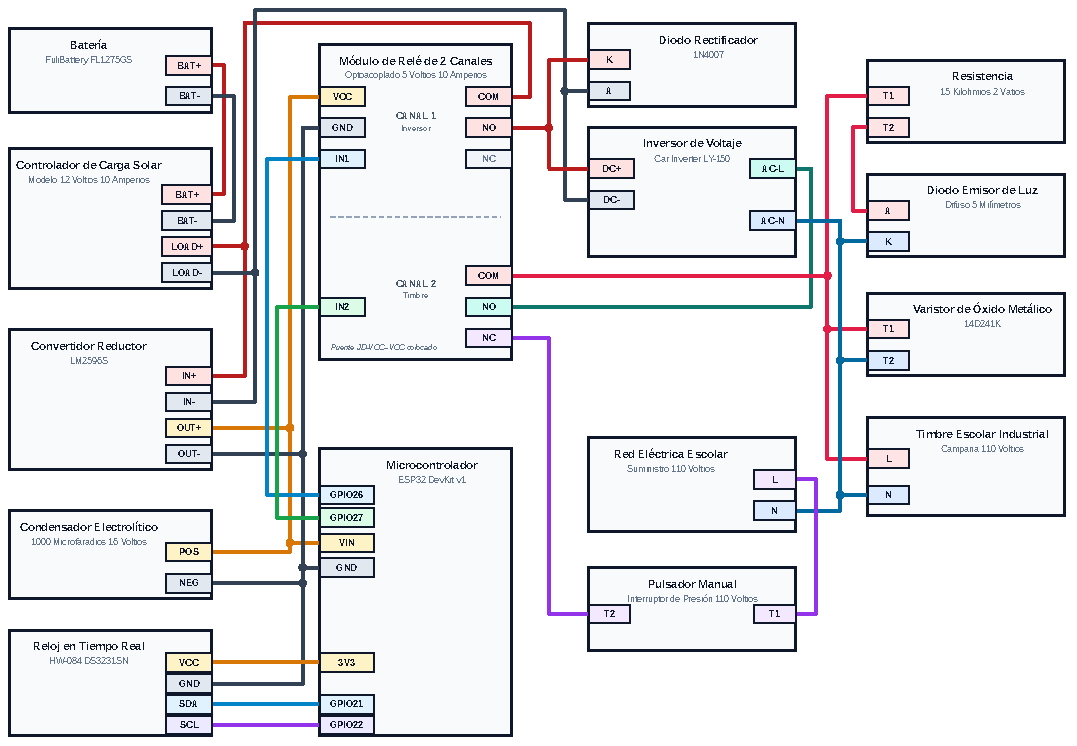
\includegraphics[width=\linewidth]{figuras/circuito-solarbell.pdf}
\caption{Esquema final del sistema de timbre con relé doble}
\label{fig:circuito}
\fuente{Circuito del sistema de timbre escolar, esquema extraído del diagrama final \cite{diagrama}.}
\end{figure}

\begin{table}[H]
\centering\small
\caption{Subsistemas y componentes principales}
\begin{tabularx}{\linewidth}{@{}P{2.52cm}P{5.35cm}Y@{}}
\toprule
\textbf{Bloque} & \textbf{Componentes identificados} & \textbf{Función} \\
\midrule
Generación y carga & Panel Powest SZYL-P30-18C de 30\,Wp y controlador PWM de 12\,V y 10\,A. & Captar energía y gestionar la carga y la salida hacia el sistema. \\
Reserva & Batería VRLA FuliBattery FL1275GS de 12\,V y 7,5\,Ah. & Almacenar energía para el control y el timbrado automatizado. \\
Regulación & LM2596S y condensador de 1000\,$\mu$F y 16\,V. & Suministrar y estabilizar los 5\,V de la rama de control. \\
Tiempo y control & ESP32 DevKit v1 y RTC HW-084 DS3231SN. & Interpretar el calendario y emitir las señales de mando. \\
Potencia & Módulo optoacoplado de dos relés, 5\,V/10\,A, e inversor LY-150 de 150\,W. & Alimentar el inversor y conmutar la línea de la campana de 110\,V. \\
Mandos de pared y radio & Pulsador EXE de 110\,V e interruptor basculante de dos terminales. & Proporcionar aviso manual y desactivar la radio Wi-Fi, respectivamente. \\
\bottomrule
\end{tabularx}
\end{table}

\clearpage
\subsubsection{Señales, potencia y software embebido}
La salida de carga de 12\,V del controlador alimenta la derivación del inversor y el regulador LM2596S. La salida regulada de 5\,V alimenta el ESP32 por \senal{VIN} y el módulo de relés. El RTC recibe 3,3\,V y se comunica por I\textsuperscript{2}C. El RTC conserva la fecha y la hora al faltar la alimentación principal \cite{ficha,diagrama}.

\begin{table}[H]
\centering\small
\caption{Mapa de señales documentadas del ESP32}
\label{tab:gpio}
\begin{tabularx}{\linewidth}{@{}P{3.20cm}P{3.70cm}Y@{}}
\toprule
\textbf{Terminal ESP32} & \textbf{Destino en el diagrama} & \textbf{Función} \\
\midrule
\senal{GPIO21} & \senal{SDA} del RTC & Datos de I\textsuperscript{2}C. \\
\senal{GPIO22} & \senal{SCL} del RTC & Reloj de I\textsuperscript{2}C. \\
\senal{GPIO26} & \senal{IN1} del relé & Mando del inversor durante la secuencia. \\
\senal{GPIO27} & \senal{IN2} del relé & Mando de la campana en cada repique. \\
\senal{GPIO33}, \senal{GND} & Interruptor de Wi-Fi & Entrada con resistencia interna: abierto deja la red propia; cerrado activa el ahorro de radio. \\
\senal{GPIO2} & LED azul de la placa & Repite el estado del relé de la campana y parpadea si el equipo no tiene hora. \\
\senal{VIN}, \senal{GND} & Salida regulada y retorno & Alimentación de la placa y referencia de control. \\
\senal{3V3}, \senal{GND} & \senal{VCC} y \senal{GND} del RTC & Alimentación y referencia del reloj. \\
\bottomrule
\end{tabularx}
\end{table}

\paragraph{Secuencia eléctrica.}
El canal 1 conecta la salida de 12\,V al inversor LY-150 durante el patrón. La ficha especifica una salida de 110\,V a 60\,Hz. El canal 2 lleva la línea del inversor al contacto común durante el repique y vuelve al contacto normalmente cerrado en reposo. En esa posición, el pulsador de pared selecciona el paso de la línea escolar hacia la campana. El esquema representa un neutro común entre la red escolar y la salida del inversor. Los dos canales cumplen funciones distintas y las fotografías no acreditan el comportamiento eléctrico de esa conexión \cite{ficha,diagrama}.

El circuito representa un condensador en la alimentación regulada, un diodo 1N4007 en la rama de corriente continua y un varistor 14D241K en la rama de la campana. Incluye un LED de prueba con una resistencia de 15\,k$\Omega$ y 2\,W. El LED aporta una indicación visual, mientras que la respuesta acústica y el consumo de la carga requieren sus propias observaciones \cite{diagrama}.

\paragraph{Firmware del ESP32.}
El firmware 0.8.0 es un único programa de Arduino en C++ para el núcleo \textit{esp32} de Espressif. La Tabla~\ref{tab:librerias} resume las librerías que usa. Las opciones de cada instalación, como la clave de la red, los pines de los relés y del interruptor y el uso del DS3231, se definen en \senal{configuracion.h}, que no se publica con el código \cite{repo}.

\begin{table}[H]
\centering\small
\caption{Librerías del firmware}
\label{tab:librerias}
\begin{tabularx}{\linewidth}{@{}P{3.3cm}Y@{}}
\toprule
\textbf{Librería} & \textbf{Uso en SolarBell} \\
\midrule
\senal{WiFi}, \senal{esp\_wifi} & Red propia SolarBell como punto de acceso, unión a la red del colegio, escaneo de redes y reposo de la radio entre balizas. \\
\senal{WebServer} & Servidor HTTP en el puerto 80 con las rutas de la Tabla~\ref{tab:api}. \\
\senal{ESPmDNS} & Anuncia el equipo como \senal{solarbell.local} en la red del colegio. \\
\senal{ArduinoJson} 7 & Lectura y escritura del horario y de las respuestas HTTP. \\
\senal{LittleFS} & Archivo del horario y archivos del historial en la flash. \\
\senal{Preferences} & Red del colegio, zona horaria y último minuto tocado. \\
\senal{RTClib} (Adafruit) & Lectura y ajuste del DS3231SN por I\textsuperscript{2}C. \\
\bottomrule
\end{tabularx}
\end{table}

El ciclo principal no se bloquea. Cada medio segundo compara la hora local con el horario aplicable a la fecha y, si coincide un evento, arranca la secuencia. La secuencia enciende el inversor, espera 2\,s a que arranque y alterna el relé de la campana según las duraciones y pausas del patrón, todas en milisegundos (de 100 a 30.000). Al terminar, apaga el inversor y anota el toque en el historial. Si el equipo no tiene hora válida, no ejecuta el horario, aunque sí atiende los toques inmediatos.

\paragraph{Interfaz HTTP del equipo.}
El ESP32 atiende peticiones JSON en \senal{192.168.4.1} dentro de su red propia, y en la IP asignada o \senal{solarbell.local} dentro de la red del colegio. Los errores responden \senal{\{"detail": "..."\}} con códigos 400, 404, 413, 422 o 500 \cite{repo}.

\begin{table}[H]
\centering\small
\caption{Rutas HTTP del firmware 0.8.0}
\label{tab:api}
\begin{tabularx}{\linewidth}{@{}P{4.6cm}Y@{}}
\toprule
\textbf{Ruta} & \textbf{Función} \\
\midrule
\senal{GET /api/status} & Versión, hora y zona, revisión del horario, próximo identificador del historial y toque en curso. \\
\senal{GET}, \senal{PUT /api/schedule} & Leer o reemplazar el horario completo, con su semana y sus fechas especiales. \\
\senal{POST /api/clock} & Fijar la hora y la zona del teléfono. \\
\senal{POST /api/ring} & Tocar ahora con un patrón. \\
\senal{POST /api/ring/stop} & Detener el toque en curso. \\
\senal{GET /api/history} & Historial paginado, con filtros \senal{limit}, \senal{before}, \senal{from}, \senal{to} y \senal{q}. \\
\senal{POST /api/history/delete} & Borrar un registro del historial. \\
\senal{GET}, \senal{PUT /api/wifi} & Estado de la red del colegio y unión a una red nueva. \\
\senal{GET /api/wifi/scan} & Redes cercanas de 2,4\,GHz. \\
\senal{POST /api/wifi/forget} & Olvidar la red del colegio. \\
\bottomrule
\end{tabularx}
\end{table}

\paragraph{Aplicación Android.}
La aplicación está escrita en TypeScript con React 19 y se empaqueta como APK con Capacitor 8 para Android 7.0 o posterior. Vite compila la interfaz, React Router organiza las seis pantallas (Inicio, Horario, Tocar, Fechas, Historial y Campana) y Tailwind CSS define los estilos. No usa servidor ni Internet: todas las llamadas pasan por un solo módulo cliente que habla con la campana con un tiempo límite de 4\,s \cite{repo}.

Mientras la campana está al alcance, la aplicación consulta \senal{/api/status} cada 2\,s, y cada 0,6\,s durante un toque, para mostrar su avance. Si deja de responder, la busca en la última IP conocida, en \senal{192.168.4.1} y en \senal{solarbell.local}, y cada 2 minutos recorre la subred. Cada cambio del horario se envía completo con \senal{PUT /api/schedule}. Si la campana no lo confirma, la aplicación vuelve a la última versión confirmada. Al conectarse corrige la hora del equipo si difiere en más de 5\,s.

\clearpage
\subsection{Pruebas del sistema}
Se realizaron cuatro pruebas. El primer ensayo usó un LED para simular el timbre y reveló un fallo. Los siguientes registros muestran el pulsador de pared y la integración del módulo de relés. La prueba definitiva se realizó con una hora programada en la Institución Educativa Cecilia de Lleras \cite{evidencia}.

\subsubsection{Prueba 1. Fallo del LED que simulaba el timbre}
\textbf{Propósito.} Comprobar si la salida de timbrado respondía a la configuración. En el montaje inicial, un LED azul hacía las veces de timbre y permitía observar el estado de la salida.

\begin{figure}[H]
\centering
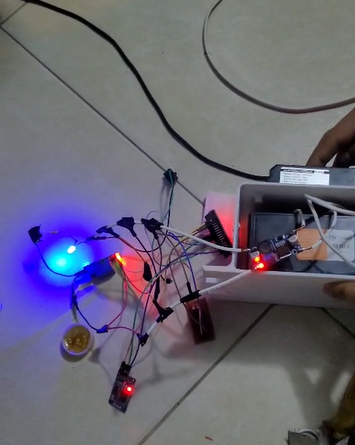
\includegraphics[width=8.9cm]{figuras/prueba-1-led.png}
\caption{LED azul encendido durante la primera prueba del montaje}
\label{fig:prueba1}
\fuente{Fotografía del equipo del proyecto \cite{evidencia}.}
\end{figure}

\textbf{Resultado observado.} La prueba fue fallida. El equipo observó que el LED se encendía independientemente de la configuración. La Figura~\ref{fig:prueba1} muestra el indicador encendido en el montaje inicial. El comportamiento reportado incumplió el criterio del ensayo, que exigía que la salida se activara de acuerdo con la configuración seleccionada.

\clearpage
\subsubsection{Prueba 2. Accionamiento del pulsador de pared}
\textbf{Propósito.} Revisar la operación del mando físico con el prototipo montado. Según el diseño, el pulsador permite accionar la campana desde la red escolar cuando el segundo relé está en reposo. Esta ruta prevé la operación manual con independencia del mando enviado desde Android \cite{ficha,diagrama}.

\begin{figure}[H]
\centering
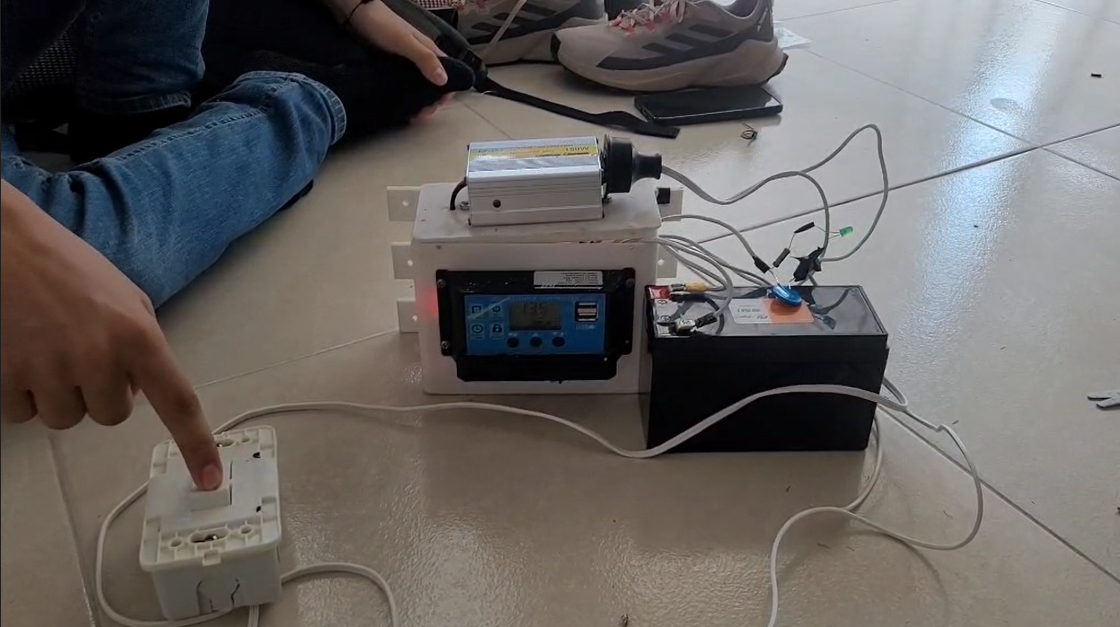
\includegraphics[width=\linewidth]{figuras/prueba-2-pulsador.png}
\caption{Pulsación del mando de pared junto al prototipo ensamblado}
\label{fig:prueba2}
\fuente{Fotografía del equipo del proyecto \cite{evidencia}.}
\end{figure}

\textbf{Resultado.} La prueba se cumplió. Con el canal 2 en reposo y la red escolar disponible, la campana sonó al pulsar el mando de pared. La Figura~\ref{fig:prueba2} muestra la pulsación junto al prototipo, con el inversor, el controlador de carga y la batería. El registro de esa respuesta está en las evidencias fotográficas \cite{evidencia}.

\clearpage
\subsubsection{Prueba 3. Integración del módulo de relés y del inversor}
\textbf{Propósito.} Examinar el conjunto de control y potencia durante una prueba del montaje. Los dos canales tienen estados distintos: uno mantiene el inversor alimentado durante la secuencia y el otro determina cuándo se aplica el toque a la campana \cite{diagrama}.

\begin{figure}[H]
\centering
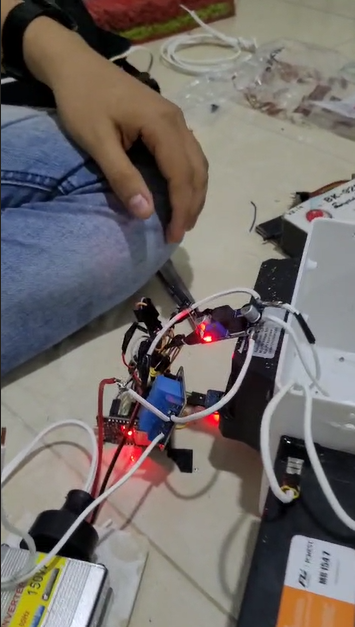
\includegraphics[width=8.45cm]{figuras/prueba-3-reles.png}
\caption{Módulo de relés y cableado próximo al inversor y a la batería}
\label{fig:prueba3}
\fuente{Fotografía del equipo del proyecto \cite{evidencia}.}
\end{figure}

\textbf{Resultado.} La prueba se cumplió. El canal 1 mantuvo el inversor encendido durante la secuencia, el canal 2 conmutó la campana en cada toque y ambos volvieron a reposo al terminar. La Figura~\ref{fig:prueba3} muestra el módulo de dos relés, el inversor y la batería durante esa prueba. La secuencia quedó registrada en las evidencias fotográficas \cite{evidencia}.

\clearpage
\subsubsection{Prueba 4. Timbrado a la hora programada en sitio}
\textbf{Propósito.} Verificar que el equipo instalado en la Institución Educativa Cecilia de Lleras ejecutara un aviso automáticamente a la hora programada.

\begin{figure}[H]
\centering
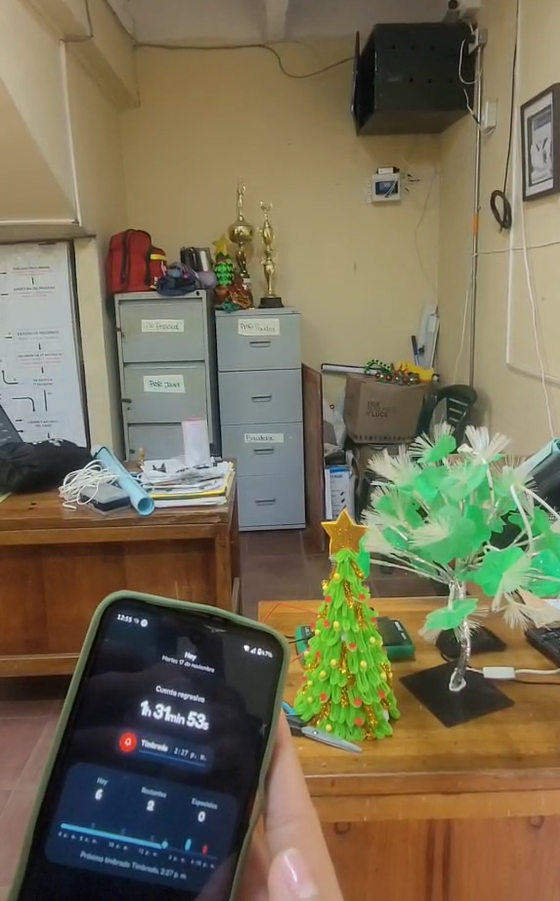
\includegraphics[width=7.8cm]{figuras/prueba-4-en-sitio.png}
\caption{Aplicación con la cuenta regresiva del timbre programado en la institución}
\label{fig:prueba4}
\fuente{Fotografía del equipo del proyecto \cite{evidencia}.}
\end{figure}

\textbf{Resultado.} En esta prueba definitiva, el equipo reportó que el ESP32 ejecutó el timbrado a la hora programada en la institución. La Figura~\ref{fig:prueba4}, tomada antes del aviso, muestra en Android la hora programada de las 2:27~p.\,m. y una cuenta regresiva de 1\,h 31\,min 53\,s \cite{evidencia}.

\begin{table}[H]
\centering\small
\caption{Síntesis de los resultados de las cuatro pruebas}
\label{tab:pruebas}
\begin{tabularx}{\linewidth}{@{}P{2.65cm}YY@{}}
\toprule
\textbf{Prueba} & \textbf{Observación registrada} & \textbf{Resultado del ensayo} \\
\midrule
1. LED & Indicador azul encendido en el montaje inicial. & Fallida. El LED se encendía al margen de la configuración. \\
2. Pulsador & Pulsación del mando de pared con la red escolar y el canal 2 en reposo. & Cumplida. La campana sonó por la ruta manual. \\
3. Integración & Módulo de relés, inversor y batería durante la secuencia. & Cumplida. El inversor se encendió, la campana conmutó en cada toque y ambos volvieron a reposo. \\
4. En sitio & Cuenta regresiva del aviso programado en Android. & Timbrado a la hora programada, reportado por el equipo. \\
\bottomrule
\end{tabularx}
\end{table}

\clearpage
\section{Conclusiones}
\begin{enumerate}
  \item \textbf{Integración del hardware (objetivo 1).} Se cumplió. El ESP32, el DS3231SN, el subsistema fotovoltaico y el módulo de dos relés forman un solo equipo. Un canal enciende el inversor durante la secuencia y el otro acciona la campana según el patrón de repiques. En reposo, el pulsador mantiene la opción de accionamiento con la red del colegio.
  \item \textbf{Control temporal (objetivo 2).} Se cumplió. El horario semanal y las fechas especiales residen en el ESP32, que los ejecuta con su propio reloj sin el teléfono ni Internet. Una fecha especial reemplaza el día completo, incluso para dejarlo sin timbres.
  \item \textbf{Gestión desde Android (objetivo 3).} Se cumplió. La aplicación pone en hora la campana al conectarse, administra el calendario, ordena y detiene toques inmediatos y consulta el historial que el ESP32 guarda de cada toque, con su origen, su resultado y el tiempo que sonó.
  \item \textbf{Documentación de las pruebas (objetivo 4).} Se cumplió. La primera prueba reveló que el LED de simulación se encendía independientemente de la configuración. Las evidencias fotográficas registran que la campana sonó con el pulsador de pared y que los dos relés siguieron la secuencia del inversor y de la campana. La prueba definitiva en la Institución Educativa Cecilia de Lleras verificó un timbrado a la hora programada, según lo reportado por el equipo.
  \item \textbf{Cambios frente a la propuesta.} La versión final sustituyó la sincronización NTP por el RTC puesto en hora desde el teléfono y el panel web por la aplicación Android en la red local, e incorporó la alimentación solar. El monitoreo por SCT-013 y la pantalla OLED quedaron fuera del alcance final. El historial de toques reemplaza en parte el registro de incidencias previsto al inicio.
\end{enumerate}

\section{Recomendaciones}
\begin{enumerate}
  \item \textbf{Usar el historial como evidencia de las pruebas.} Comparar cada registro con la hora esperada, el número de toques, la duración y la respuesta audible. El historial prueba que el ESP32 dio la orden, no que la campana sonó, por lo que conviene acompañarlo con un video breve del mismo momento.
  \item \textbf{Probar el calendario en días representativos.} Incluir un día hábil normal, una fecha especial con horario propio y una fecha especial sin avisos. Repetir un evento con el interruptor de Wi-Fi en ahorro y consultar la programación y el historial al recuperar la comunicación.
  \item \textbf{Medir la operación energética.} Registrar el consumo en reposo, el consumo con la radio apagada, la duración de los repiques y el comportamiento de la batería en jornadas representativas. Usar esas mediciones para estimar autonomía y evaluar el aporte del panel.
  \item \textbf{Revisar la etapa de potencia del equipo instalado.} Encargar a personal competente la revisión de la conmutación entre fuentes, el neutro representado en el esquema, las protecciones y el montaje físico.
\end{enumerate}

\clearpage
\section{Trabajos futuros}
\paragraph{Confirmación de carga y registro de avisos.}
Evaluar la incorporación del sensado de corriente planteado al inicio, con calibración para la campana real. Vincular la confirmación de la carga con el historial de timbrados permitiría identificar cuándo se ejecutó un aviso sin la respuesta eléctrica esperada.

\paragraph{Validación de autonomía y manejo de eventos.}
Medir el consumo y la recarga bajo patrones escolares y condiciones solares variadas. Complementar la evaluación en la institución con ensayos de pérdida de alimentación, puesta en hora posterior al reinicio y manejo de solicitudes simultáneas.

\paragraph{Gestión y supervisión.}
Evaluar controles de acceso para la edición del horario, ya que hoy la única protección es la clave de la red, y una forma de exportar el horario y el historial como respaldo fuera del equipo. Añadir avisos locales sobre las condiciones de funcionamiento que requieran revisión.

\section{Bibliografía}
\begingroup
\small
\renewcommand{\section}[2]{}
\begin{thebibliography}{99}
\setlength{\itemsep}{3pt plus 0.5pt}
\bloquebiblio{propuesta}{Equipo del proyecto. \textit{Propuesta inicial de Proyecto de Aula Semestral: Sistema inteligente de automatización de timbre escolar con monitoreo activo de fallas y diagnóstico de corriente (SCT-013)}. Universidad de Córdoba.}{Documento de trabajo.}
\bloquebiblio{ficha}{Ortiz Rodríguez, A. F., Hernández López, N. J., Otero Pineda, J. E. y Doria Guevara, J. C. (2026). \textit{Fichas de hardware y software. SolarBell}. Universidad de Córdoba.}{Documento técnico del proyecto.}
\bloquebiblio{diagrama}{Equipo SolarBell. \textit{Circuito del sistema de timbre escolar: relé doble}.}{Diagrama eléctrico del prototipo.}
\bloquebiblio{evidencia}{Equipo SolarBell. \textit{Registro de las pruebas del prototipo y de la instalación en la Institución Educativa Cecilia de Lleras}.}{Evidencias fotográficas de las cuatro pruebas, con el sonido del pulsador y la secuencia de los relés.}
\bibitem{repo} Equipo SolarBell. (2026). \textit{SolarBell}, rama \senal{main}, revisión \senal{0adeb14}: firmware 0.8.0 y aplicación Android. \href{https://github.com/AndresOrtizJDK/SolarBell/tree/0adeb14514f4e0b15457052f21800002322fbb43}{Repositorio en GitHub}.
\bibitem{mahmood} Mahmood, R. Z. (2022). High Accurate Automatic School Bell Controller Based On ESP-32 Wi-Fi. \textit{Technium}, 4, 126--144. \href{https://doi.org/10.47577/technium.v4i10.7929}{DOI 10.47577/technium.v4i10.7929}.
\bibitem{gaceno} Buitrago Porras, A. F., Gamba Cordon, G. S., Mora Novoa, L. J. y Polania Daza, R. A. (2024). \textit{Diseño y construcción de un timbre automatizado para la Institución Educativa San Luis de Gaceno}. \href{https://repositorio.colegiosanluisgaceno.edu.co/proyecto-implementacion-de-una-pagina-web-corporativa-graficas-san-vicente/}{Repositorio institucional}.
\bibitem{flores} Flores Cortez, O. O. y Cornejo, J. R. (2025). Desarrollo e implementación de un prototipo electrónico de timbrado automatizado en escuelas públicas de El Salvador. \textit{Entorno}, 80. \href{https://doi.org/10.5377/entorno.v1i80.21030}{DOI 10.5377/entorno.v1i80.21030}.
\bibitem{badillo} Badillo Rincón, J. S. (2024). \textit{Prototipo de sirena automatizada utilizando tecnologías Internet de las Cosas (IoT) como estrategia para optimizar el cumplimiento de la jornada escolar en instituciones educativas}. Universidad Popular del Cesar, seccional Aguachica. \href{http://repositorio.unicesar.edu.co/items/8a9ad412-bb9a-4cf4-b1f6-d2a827a3a118}{Repositorio institucional}.
\bibitem{yepes} Yepes Mercado, D. A. y Gómez Polo, I. A. (2025). \textit{Timbre automatizado con luces LED para estudiantes sordos}. Universidad de Córdoba. \href{https://repositorio.unicordoba.edu.co/handle/ucordoba/9186}{Repositorio institucional}.
\end{thebibliography}
\endgroup

\clearpage
\seccionsinnumero{Anexos}
\begin{description}
  \item[A. \enlaceanexo{https://drive.google.com/file/d/1LomUXdingYTk7quJXPIZwikhOhr79yUv/view?usp=sharing}{Manual del usuario.}] Operación diaria de la campana desde la aplicación Android, con capturas de cada pantalla.
  \item[B. \enlaceanexo{https://drive.google.com/file/d/1DUVH0cu2mJqsOCFwGHQkQuvZdIaeXf2i/view?usp=sharing}{Manual del sistema.}] Instalación, configuración, firmware, pruebas, diagnóstico y mantenimiento.
  \item[C. \enlaceanexo{https://drive.google.com/drive/folders/1H0iyxZqXhvPPEtefXjU5ecN3YwtofA8R?usp=sharing}{Evidencias fotográficas.}] Las fotografías del cuerpo del informe muestran cada prueba. La carpeta completa incluye el registro del sonido del pulsador y de la secuencia de los relés.
  \item[D. \enlaceanexo{https://github.com/AndresOrtizJDK/SolarBell}{Códigos fuente.}] El firmware del ESP32 y la aplicación Android. La versión descrita en este informe es la revisión \senal{0adeb14} \cite{repo}.
\end{description}

\end{document}
